\documentclass{standalone}
\usepackage{tikz}
\usetikzlibrary{automata,positioning,arrows,shapes,decorations,calc,
arrows.meta,fit}
\usetikzlibrary{decorations.pathmorphing}
\usetikzlibrary{decorations.pathreplacing}
\usetikzlibrary{decorations.shapes}
\usetikzlibrary{decorations.text}
\usetikzlibrary{decorations.markings}
\usetikzlibrary{decorations.fractals}
\usetikzlibrary{decorations.footprints}

\tikzset{
roundnode/.style={rectangle, draw=black, very thick, text width=40mm, minimum height=1cm},
phasenode/.style={rectangle, draw=black, very thick, text width=3cm, minimum height=1cm},
phasenodeBis/.style={rectangle, draw=black, very thick, minimum width=8cm, minimum height=5cm},
>={Latex[width=2mm,length=2mm]},
base/.style = {rectangle, rounded corners, draw=black,
                         minimum width=4cm, minimum height=1cm,
                         text centered, font=\sffamily},
%every picture/.style={/utils/exec={\sffamily}}
every edge quotes/.append style={font=\scriptsize, align=center, auto}% style for edge labels
}

\begin{document}
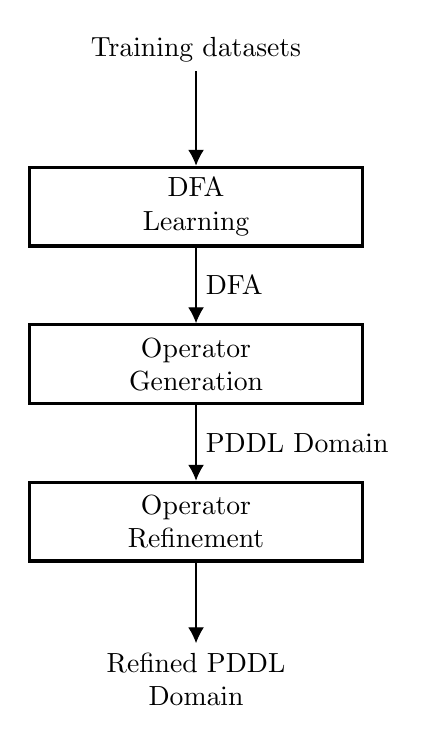
\begin{tikzpicture}[node distance=1.5cm, align=center]

%Automaton nodes
\node[text width=3cm] (gen) at(0,0)  {Training datasets};
\node[roundnode] (gram) at(0,-2)  {DFA\\Learning};
\node[roundnode] (pddlLearn) at(0,-4)  {Operator\\Generation};
\node[roundnode] (refinement) at(0,-6)  {Operator\\Refinement};

% \node[text width=5cm] (input) at(0,2)  {Actions name and\\ Observable Predicates};
\node[text width=3cm] (output) at(0,-8)  {Refined PDDL Domain};

% \draw[->] (input) -- (gen);
\draw[->] (gen) -- (gram) ;
\draw[->] (gram) --node[right] {DFA} (pddlLearn) ;
\draw[->] (pddlLearn) --node[right] {PDDL Domain} (refinement) ;
\draw[->] (refinement) -- (output) ;

\end{tikzpicture}
\end{document}
